\documentclass[12pt,twoside, parskip=half, headsepline=on, chapterprefix=true, draft=off]{scrbook}

\usepackage[english]{babel}
\usepackage[T1]{fontenc}
\usepackage[utf8]{inputenc}
\usepackage{lmodern}
\usepackage{graphicx}
\usepackage{amsmath}
\usepackage{caption}
\usepackage{color}
\usepackage{adjustbox}
\usepackage[breakable,skins]{tcolorbox}

\renewcaptionname{english}{\chaptername}{Module}

\definecolor{shadecolor}{gray}{0.5}

%\usepackage{hyperref}
%\hypersetup{colorlinks=true, urlcolor=[rgb]{0.25,0.41,0.88}, linkcolor=[rgb]{0.25,0.41,0.88}, pdftitle=Course, pdfauthor=Niko, pdfsubject=, pdfkeywords=}
\usepackage{scrlayer-scrpage}

\ihead{CECAD -- IIAM} 
\chead{} 
\ohead[]{\headmark} 
\renewcommand*{\chapterpagestyle}{scrheadings}
\pagestyle{scrheadings}

\newcounter{taskcounter}
\newenvironment{taskbox}[1]{%
	\begin{tcolorbox}[enhanced,breakable,colframe=red!75!black]%
	\begin{addmargin*}[1em]{1em}%
			\refstepcounter{taskcounter}%
			\vspace{0.5cm}\textbf{Exercise} \textbf{\thechapter.\arabic{taskcounter}:} #1%
			\\\rule[0.9em]{\linewidth}{1pt}%
}{%
	\end{addmargin*}%
	\end{tcolorbox}%
}

\usepackage{natbib}


%% Start Document

\begin{document}

% title 
\title{An Introduction to Image Analysis in Microscopy}
\subtitle{CECAD Imaging Facility Course, v1.1} 
\author{Nikolay Kladt}
\date{\today}
\publishers{Imaging Facility\\Cluster of Excellence -- Cellular Stress Responses in Aging-Associated Diseases\\University of Cologne}

\maketitle

\tableofcontents

% Module 1: Publishing microscopy data (The Basics)
%\chapter{Publishing original microscopy data}

In this module, we will work through some necessary basics of image processing and explore common ways to visualize microscopy data. After this module, you should feel comfortable working with your images in Fiji and be able to use this knowledge to prepare your data for publication.

Digital images are ubiquitous and nearly everybody is used to taking pictures with a digital camera or smart-phone and also storing and processing these images. The same way that digital imaging has replaced analog cameras in our daily lives, light microscopes have transformed to digital imaging systems\footnote{In this course, we do not discuss the technologies that actually generate digital images in microscopes. If you want to learn about various microscopy techniques, we recommend looking at the online iBiology Microscopy Course (www.ibiology.org/ibioeducation/taking-courses/ibiology-microscopy-course.html, 25-02-2015)}. Even the most simple light microscopes are usually equipped with a digital camera and a screen to display, take and store images - also allowing quick and simple image processing tasks without the need for additional software (e.g. brightness \& contrast adjustments, white balancing). More complex light microscopes, such as confocal laser scanning microscopes (CLSM), already require sophisticated software interfaces to set up imaging parameters and visualize the results. Finally, there are also types of microscopes that depend on digital image processing (e.g. stochastic optical reconstruction microscope, STORM or single plane illumination microscopy, SPIM).

As a result of these advancements, modern digital microscopy offers more than just 'pretty pictures' - there are many imaging techniques that rely on computational analysis as well as methods for image enhancement, restoration and quantitative analysis. Modern microscopy cannot be understood without the basics of digital images and digital image processing. This knowledge is not only essential to make full use of the capabilities, but also to understand limitations -- a very important prerequisite to maintain scientific validity.

\minisec{Raster and vector images}
Typically, most pictures you work with (scanned documents, photos taken with a digital camera, pictures found on the web) are raster graphics (see Fig. \ref{fig:bitmap-graphics}). This means that these images are made up of a grid of \emph{pixels} (picture elements). Each pixel has a value that represents some property of the image (usually brightness). The range of this value is called \emph{bit-depth} and determines possible values at each pixel. Sometimes, the term \emph{bitmap image} is used for a raster image. For example, the image shown in figure \ref{fig:bitmap-graphics} illustrates a raster image with 420 x 420 pixels and a bit-depth of 1 byte. Therefore, we have a total of 176400 pixels, multiplied with 1 byte taking up a total of 172 kilobytes disc space. As you can see, the number of pixels and the bit-depth affect the required disc space. Additionally, we cannot easily change the size of the image; enlarging causes the image to look 'pixelated' or we have to use interpolation techniques to estimate the value of added pixels. Decreasing the number of pixels in the image might result in a loss of image features. There are plenty of commercial and open-source programs to work with raster images; representative software packages are Adobe Photoshop (Adobe Inc., San Jose) and GIMP (GNU Image Manipulation Program, The GIMP team, http://gimp.org).

\begin{figure}[!ht]
	\centering
		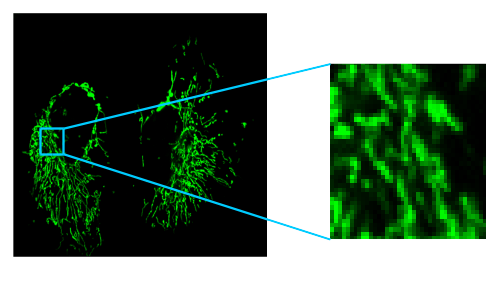
\includegraphics[width=0.60\textwidth]{mod1-publishing/figures/bitmap-graphics.png}
	\caption{Fluorescent labeled mitochondria in HeLa cells. THis image shows that raster graphics are made up of pixels that become clearly visible when zoomed.}
	\label{fig:bitmap-graphics}
\end{figure}


In contrast, vector graphics are not made up of a bitmap. Instead, they are based on geometrical shapes such as lines, curves, polygons or other shapes that are based on mathematical expressions. Therefore, these images can be scaled without a loss in image quality and typically use less disc space than raster images. Especially when the scaling of lines, text or other image content might change, it makes sense to use vector graphics (e.g. figures for a manuscript, scientific poster). Similar to the editors for raster images, there are plenty of vector graphics programs; representative examples are Adobe Illustrator (Adobe Inc., San Jose) and Inkscape (The Inkscape team, http://www.inkscape.org).

Often, programs support the conversion between raster and vector graphics. These are called \emph{rasterization} and \emph{vectorization}. Usually, vector graphics programs allow you to include raster-graphics without conversion.

Let's say you're done for the day and want to submit another great manuscript to Nature (Nature Publishing Group). Nature has detailed requirements on how your figures should be prepared for print (http://www.nature.com/nature/authors/gta/3c\_Final\_artwork.pdf, as of 08.10.2014). According to their guide, they prefer vector graphics for text and line-art. We will revisit the Nature figure requirements as we go along discussing properties of digital images!

\begin{verse}
\emph{Can you explain why journals prefer vector graphics for text and line-art?}
\end{verse}

\section{Pixels, spatial resolution and sampling frequency}
\label{sec:mod1-samplingrate}

It is important to remember that our microscopes have an optical resolution\footnote{For this course, we assume that you have a basic understanding why microscopes have an optical resolution and on which parameters the optical resolution depends.} that defines the ability to resolve details of the specimen. 

Limited by the optical resolution, the number of discrete pixels in a digital image then determines the spatial resolution. The number of pixels is usually called the sampling frequency (or sampling interval). This simply means that the spatial resolution depends on the number of pixels within given physical dimensions and that the maximum spatial resolution is limited by the optical resolution\footnote{This is only partially true -- we can theoretically build a microscope where the detector is the limiting factor. In general, the detector is chosen to match the optical resolution; and all internal microscope components involved in generating the digital image have to be matched as well.}. It is important to note that each pixel represents the average response of the optical system measured at a point within an area that is specified by the characteristics of our optical system. 

In a typical confocal microscope (not camera based), we can choose the number of pixels with which we want to sample the acquired image. A change in the pixel number obviously changes the size of the pixel and therefore also the area of which the average response is obtained. Choosing the wrong sampling frequency is a typical pitfall in microscopy, especially when zoom controls are used. If we sample inadequately, details can be lost. Oversampling is usually not critical, we just increase the amount of data we have to handle and we have to know that we oversample. Fortunately, sampling theory tells us exactly which sampling interval (pixel size, pixel number) is required to optimally represent the biological specimen given our optical resolution (the famous \emph{Nyquist theorem} states that we require a sampling interval $\geq$ twice the highest spatial frequency in our specimen and the highest frequencies we can observe are physically limited by our optical resolution). 

This raises the question why our microscopes even allow us to change the sampling frequency and not always simply operate at the diffraction-limited configuration. The reason is, that there are many experimental situations where it is desirable to intentionally lower our spatial resolution. Basically, we have to make a trade-off between the required resolution and imaging speed, amount of light collected at each pixel, photo-toxicity or other experimental parameters. The important thing is that we are aware of the fact that we under-sample for whatever reasons we have.

The limited number of discrete pixels in an image acquired with a microscope has serious consequences when you create figures for a manuscript. Publishers often require a certain number of pixels per cm (inch) to create high-quality figures and unfortunately, they leave it up to you to adjust your figures. However, they usually ignore the fact that you only have a limited number of pixels in your original data. One option you have is resampling your original data to change the number of pixels. Another option is to show pixels enlarged -- leading to a pixelated view of your data.

\subsection{Resampling Images}

Resampling an image changes the original data; the number of pixels is either increased or decreased (enlarging, shrinking). In comparison, using the zoom tool (icon magnifying glass) just increases or decreases the size of the pixels on your screen without resampling. Similar to other programs, Fiji also allows you to change the size of the canvas (the space on which your image is drawn, see Figure \ref{fig:adjust-canvas-dialog}. If you adjust the canvas size \texttt{[Image > Adjust > Canvas Size]}, the image is either cut (pixels outside the canvas size are cut off) or a margin is added where added pixels usually have the background color (zero value). 

\begin{figure}[!ht]
	\captionsetup{justification=centering}
	\centering
		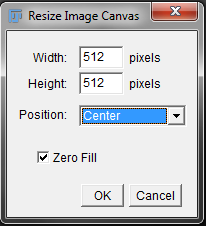
\includegraphics{mod1-publishing/figures/adjust-canvas-dialog.png}
		\caption{Adjust Canvas Size Dialog.}\label{fig:adjust-canvas-dialog}
\end{figure}

As you saw above, we determine the number of pixels during image acquisition according to our needs and the limits of the microscope. However, when you prepare your data for a presentation, poster or manuscript you will usually have to scale your original data. Before we discuss best practices and look at an example, we will introduce important basic terminology.

\minisec{Image resolution outside microscopy}

In printed images and in document scanners, resolution is often given in \emph{DPI (Dots Per Inch)}, the number of dots within a line that spans 1 inch (2.54 cm). Computer screen, tablet or phone resolution is typically given in \emph{PPI (Pixels Per Inch)}, the number of pixels within a line that spans 1 inch. Confusing, DPI is often used when PPI would be better, and even more confusing, one printer dot is usually not equal to one pixel! 

As we learned in section \ref{sec:mod1-samplingrate}, knowing the number of pixels is not sufficient to define the resolution -- pixel size (sampling rate, distance of pixels, ..) is necessary as well. This is also true for consumer products such as digital cameras, smartphones or flatscreen TVs. Knowing that a Full HD TV is capable of displaying 1920 x 1080 pixels presents no information about the size of each pixel. An 18 mega-pixel camera that is able to generate photos with 5184 x 3456 pixels also has no resolution associated. For screens, we can calculate the PPI by dividing the number of pixels by the size of the screen. For example, a 40'' Full HD TV would have 55.07 PPI, an IPhone 5 about 326 PPI (4'', 1640 x 1136 pixels but two dots per pixel!), an Amazon Kindle Paperwhite 212 PPI (6'', 1024 x 758). 

High quality photo printing requires about 200-300 PPI. With the number of pixels of our digital camera, we can calculate the maximum size of a high-quality print. For example, an 18 mega-pixel camera print with at least 200 PPI: 

\begin{quotation}
	18 mega-pixel = 5184 x 3456 pixels, divided by 200 PPI results in a print of about 65 x 43 cm (1 inch = 2.54 cm).
\end{quotation}

Publishers usually require that you submit your figures in 300-600 DPI (meaning PPI), depending on the content (e.g. see the requirements of Nature\footnote{http://www.nature.com/nature/authors/gta/3c\_Final\_artwork.pdf, as of 08.10.2014} or PNAS\footnote{http://www.pnas.org/site/misc/digitalart.pdf, as of 04/03/2015}). This already determines the maximum size of your (sub)figure given available pixels. 

\begin{taskbox}{Resampling Example - No Interpolation}

\begin{enumerate}
	\item Open the file resampling-test.tiff in /module1/data. This is a 20x20 pixel black-and-white (binary) image. Use the magnification tool to zoom to the maximum magnification. You should now see a one pixel wide and a two pixel wide vertical white line and a 1px diagonal line. 
	\item Before we perform image manipulations, we duplicate the original image for convenience \texttt{[Image > Duplicate]}.
	\item Go to [Image > Adjust > Size], you should see a dialog as shown in figure \ref{fig:adjust-size-dialog}.
	
	\begin{minipage}[t]{\linewidth}
		\begin{center}
		\adjustbox{valign=t}{%
			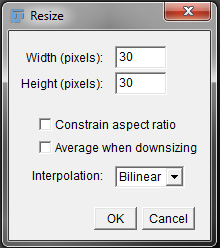
\includegraphics[width=0.3\textwidth]{mod1-publishing/figures/adjust-size-dialog.png}%
		}
		\medskip
		\captionof{figure}{Adjust Size Dialog.}\label{fig:adjust-size-dialog}
		\end{center}
	\end{minipage}
	
	\item Perform a resize to 30 x 30 pixels (150\% size), with no interpolation, and compare the result with the original figure. Use the \texttt{Line-Tool} (see fig. \ref{fig:line-tool}) to measure the width of both vertical lines. You should observe that one line was not scaled while the other was scaled to 150\%.
	
	\begin{minipage}[t]{\linewidth}
		\begin{center}
		\adjustbox{valign=t}{%
			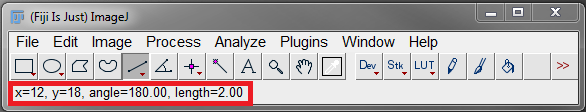
\includegraphics[width=0.7\textwidth]{mod1-publishing/figures/line-tool.png}%
		}
		\medskip
		\captionof{figure}{Line tool selection and values.}\label{fig:line-tool}
		\end{center}
	\end{minipage}
	
	\item Try other values for the resizing and observe the results.
\end{enumerate}

\end{taskbox}

\begin{taskbox}{Resampling Example - With Interpolation}

\begin{enumerate}
	\item Again, work on a duplicate of the resampling-test.tif image.
	\item Adjust the size to 150\% with interpolation set to 'Bilinear'. Use the \texttt{Point-Tool} and move the mouse over the image. On the bottom of the Fiji bar, you should see the mouse position in pixels and the value of the current pixel (Figure \ref{fig:pixel-position}).
	
	\begin{minipage}[t]{\linewidth}
		\begin{center}
		\adjustbox{valign=t}{%
			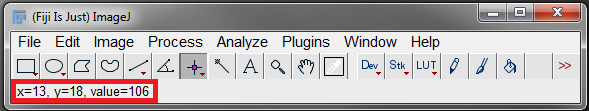
\includegraphics[width=0.7\textwidth]{mod1-publishing/figures/pixel-position.png}%
		}
		\medskip
		\captionof{figure}{Pixel position and value.}\label{fig:pixel-position}
		\end{center}
	\end{minipage}
	
	\item While the interpolation helps to visually estimate the 150\% re-sampling in the vertical and diagonal lines, you can see that the original data has been changed.
	\item Try other values for the resizing and observe the results.
\end{enumerate}
\end{taskbox}

As you should have observed, the bilinear interpolation leads to gray values appearing in the previously black-and-white image. Fiji supports the bilinear and the bicubic interpolation. Both interpolation algorithms sample pixel values surrounding each pixel to calculate the pixel value at the given position\footnote{For more information, Wikipedia has entries for bilinear and bicubic interpolations.}. 

Let us go back to our main question of making figures for a manuscript that we want to publish. PNAS recommends a minimum resolution of 300 DPI for color images and further suggests not to use interpolation when changing the size of the image. What should we do with our microscope images? Following guidelines should help you decide what to do:

\begin{itemize}
	\item Best practice: \emph{no image resampling ever} (e.g., see recommendations of the Journal of Cell Biology). Usually, you have enough pixels (>1000 x 1000 pixels), allowing you to choose an image size within your figure that is sufficient. For example, a 1000 x 1000 pixel image at 300 DPI results in about 130 pixels/cm -- you can choose a single column of 89 mm width (Nature requirements again) to display this image. If you then adjust the size of the image in your graphics software, you will only increase/decrease the size of each pixel (like the zoom tool) without resampling.
	\item Never resample more than once during image processing.
	\item Do the resampling at the end, after all other image manipulations and quantifications have been done.	
	\item Report any resampling procedures, including the original image size, pixel dimensions and the interpolation method.
	\item Most journals allow supplementary original data - a good way to present the raw, unfiltered data. Also, there is increasing interest to provide platforms that allow you to publish raw data (e.g. Figshare\footnote{www.figshare.com, an online digital repository - free to upload and free to access; as of 13.10.2014})
	\item Most important if you really have to resample: Convince yourself (and your lab-mates) that the original image and the re-sampled image convey the same information.
\end{itemize}

Fiji also has the option to directly interpolate the image to a given size and DPI (PPI!) using \texttt{[Image > Adjust > Scale To DPI]}. Using this function, you do not have to calculate the values yourself using the \texttt{[Adjust Size]} function (Fig. \ref{fig:scale-to-dpi-dialog}).
\begin{figure}[!h]
	\centering
		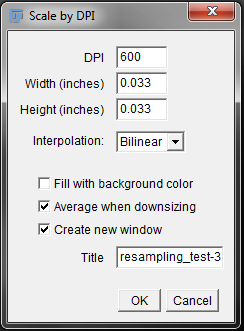
\includegraphics[width=0.3\textwidth]{mod1-publishing/figures/scale-to-dpi-dialog.png}
	\caption{Scale to DPI dialog.}
	\label{fig:scale-to-dpi-dialog}
\end{figure}

\section{Bit-Depth \& Computer Number Representations}

We already introduced the term bit-depth that describes the range of values that can be represented at each pixel. When we refer to the possible values of each pixel, we use the terms brightness or intensity in the course context. It is very likely that you already encountered the words \emph{bit}, \emph{bits}, (kilo-, mega-, giga-)\emph{bytes} somewhere: 32/64-bit computers, 8/16-bit microscopy images or 50 Mbit/s internet connection speed.

A \emph{bit} is the elementary unit of binary numbers and its possible values are 0 and 1. Electronic devices code and store information with binary numbers because binary states (0 and 1) can easily be implemented in electronics\footnote{While this statement is true, it leaves out any details. However, there are plenty of resources on the web if you are really interested why and how bits are used.}. If you have two bits, you can represent 4 different states (00, 01, 10, 11). In general, if you have \textbf{n} bits, you can represent \textbf{2\textsuperscript{n}} different states. Therefore, 8 bits allow you to represent 256 (2\textsuperscript{8}) different brightness values and 16 bits already 65536 (2\textsuperscript{16}) different values. The higher the bit-depth of our image, the more gray-levels can be represented between black (0) and white (Maximum value). One \emph{byte} consists of 8 bits (historic and convenience reasons). One kilobyte is a multiple of a byte, either 1000 bytes or 1024 bytes; this can be confusing and usually depends on the context. The same is true for further multiples, such as mega-, giga-, tera-, and petabytes.

Similar to choosing an appropriate pixel size (see section \ref{sec:mod1-samplingrate}-samplingrate}), we also have to make choices regarding the pixel intensity values during acquisition:
\begin{itemize}
	\item \emph{Bit-depth:} During image acquisition, we round the brightness values found in our samples into a certain number of levels that our chosen bit-depth can represent. For example, if we have 300 distinct brightness levels in our sample and we choose an 8-bit bit-depth, we cannot represent all 300 values (we only have 256 levels!). In this case, the 300 distinct values are rounded to the nearest level that can be represented. Pixels that have different intensities in our sample get rounded to the same values and the differences are lost. In practice, we do not worry about rounding errors during image acquisition -- we usually only have to make the choice between a low bit-depth (8-bit) and a higher bit-depth (12/16-bit). This is discussed in section \ref{sec:bitdepth-choice}. However, rounding errors can present problems during image processing. This is discussed in later chapters.
	\item \emph{Data saturation / clipping: } When you take images on a microscope, you usually set the laser output power, detector gain and detector offset for every image. The reason is that whatever bit-depth we chose, we want the brightest pixels just around the maximum value that can be represented by our bit-depth range and the darkest pixels just around zero. If we use the wrong settings and pixels are saturated/clipped, we loose information about the brightest and darkest parts of our sample. This can prevent further analysis of our data! Clipping can also occur during image processing as you will see in a few minutes.
\end{itemize}

The most common image bit-depths that you can generate with microscopes and that are supported in Fiji are:
\begin{itemize}
	\item 8-bit images that can display 256 gray levels with whole numbers (Integers).
	\item 16-bit images that can display 65536 different gray levels with whole numbers (Integers).
\end{itemize}

In addition, there is a 32-bit image format that allows you to display 2\textsuperscript{32} gray levels with real numbers. However, this format is a little bit more tricky to use as many functions in Fiji do not handle this bit-depth properly.

When you prepare your figures, bit-depth is usually not a big issue. However, you have to be careful when you export/import images using various file formats -- some common file formats only support 8-bit bit-depth and you have to make sure that you convert appropriately.

\begin{taskbox}{Bit-Depth Conversion}
\begin{enumerate}
	\item Open the image beads.tif from mod1-publishing/data using \texttt{[File > Open]}. Duplicate the image with \texttt{[Image > Duplicate...]}. Choose the line selection tool and draw a line through one of the bright spheres in the image (Fig. \ref{fig:line-roi-example}).	
	
	\begin{minipage}[t]{\linewidth}
		\begin{center}
		\adjustbox{valign=t}{%
			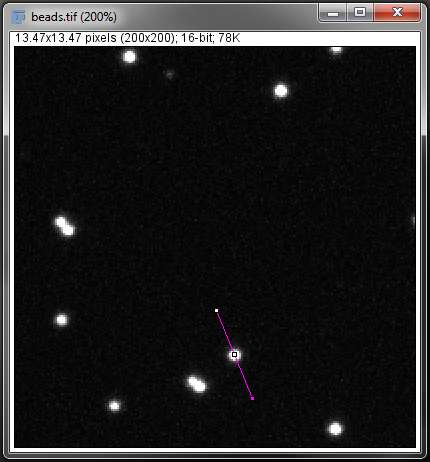
\includegraphics[width=0.5\textwidth]{mod1-publishing/figures/line-roi-example.png}%
		}
		\medskip
		\captionof{figure}{A line ROI through one of the beads.}\label{fig:line-roi-example}
		\end{center}
	\end{minipage}
	
	\item In the next step, we will look at the intensity (brightness) distribution along this line. For this, do \texttt{[Analyze > Plot Profile]} (Fig. \ref{fig:plot-profile-example}). You should observe that the gray value (y-axis) ranges from 0 to 65535 and that the curve looks cut at the upper end - this means that we have \emph{saturated} pixels, i.e. we cannot resolve any differences between these saturated pixels although the shape of the curve would suggest intensity changes. The [Plot Profile] function allows you to list (show), save and copy the values. If you click on \texttt{[Live]}, you can change the line ROI and the plotted profile will update. Try the update by drawing a line somewhere on the background and then again through a bead. Turn the live mode off again by another click on the button. 

\begin{minipage}[t]{\linewidth}
		\begin{center}
		\adjustbox{valign=t}{%
			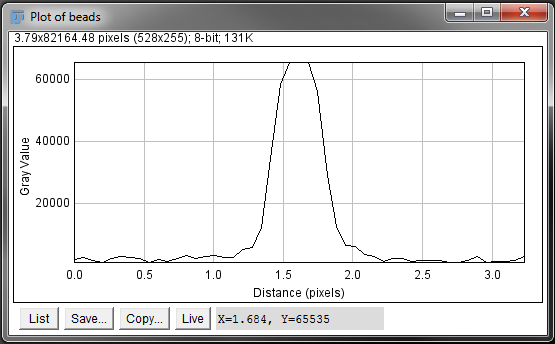
\includegraphics[width=0.5\textwidth]{mod1-publishing/figures/plot-profile-example.png}%
		}
		\medskip
		\captionof{figure}{Intensity profile of the line.}\label{fig:plot-profile-example}
		\end{center}
	\end{minipage}

\item Now, we convert the 16bit image to 8bit. First, we make sure that we scale during conversion by \texttt{[Edit > Option > Conversion]}. Then, we use \texttt{[Image > Type > 8-bit]} to convert the image. Make sure that the line ROI is still there and perform the plot profile function again. A second window pops up. Compare the plot profiles of the 8-bit and the 16-bit images. The conversion modified the brightness value (y-value). While the profiles are similar, the scaling is different. The image is scaled according to following equation:
	\[I_{8bit}=\frac{I_{16bit}(x,y)-min(I_{16bit}(x,y))}{max(I_{16bit}(x,y))-min(I_{16bit}(x,y))}*2^8
	\]
with:\\
I\textsubscript{16bit}(x,y): 16bit image\\
I\textsubscript{8bit}(x,y): 8bit image\\
max(I\textsubscript{16bit}(x,y)): maximum value of 16bit image\\
min(I\textsubscript{16bit}(x,y)): minimum value of 16bit image\\
\item Convert the image back to 16-bit and check the intensity values again. In this case, the intensity values are not increased. 
\item The conversion actually looks at the data as it is displayed. Adjust the brightness and contrast to an extreme value using \texttt{[Image > Adjust > Brightness/Contrast...]} (contrast slider to the right edge). Convert the image to 8-bit again. Look at the profile of a bead. You should see that the image only consists of 2 intensities: 0 and 255. As you saw, it is important to reset the brightness and contrast display before converting the image.
\end{enumerate}

\end{taskbox}

\subsection{Choice of Bitdepth}
\label{sec:bitdepth-choice}

The choice whether to use a low or high bit-depth depends on the application. Of course you could always use the maximum bit-depth available (to be on the safe side). However, this increases the amount of data you acquire. For example, going from 8-bit to 16-bit doubles the required harddisk space. In addition, image processing might be much slower as well! A typical application where a lower bit-depth is sufficient is where you have a very bright signal (signal-noise ration very good) and you just want to identify cells (vesicle, nuclei, ...) for counting or shape analysis. On the other hand, if you want to analyze bright regions as well as darker regions, or need precise intensity comparisons (e.g. for protein density measurements), a higher bit-depth is recommended.

\section{Image Dimensions}

Up to now, we just looked at 2-dimensional images, where each pixel \emph{p} can be identified by its spatial coordinates, its position along both axes \emph{p(x,y)}. In microscopy, we often deal with more dimensions, common scenarios are:

\begin{itemize}
	\item \textbf{3D z-stacks:} A single acquisition of a 3D volume. The additional dimension is the depth of the section. Each pixel \emph{p} can be identified by \emph{p(x,y,z)}.
	\item \textbf{3D time-series:} A sequence of 2D image acquisitions. The additional dimension is the time of the acquisition. Each pixel \emph{p} is identified by \emph{p(x,y,t)}. 
	\item \textbf{3D multi-channel images:} A 2D image is acquired with >1 color channel (multiple fluorophores). The additional dimension is the color. Each pixel is identified by \emph{p(x,y,c)}.
	\item \textbf{4D images:} a combination of 4 already discussed dimensions: z-stacks with multiple color channels, sequence of z-stacks over time or 2D multicolor image over time.
	\item \textbf{5D images:} a combination of all discussed dimensions: sequence of z-stacks with multiple color channels over time. Each pixel \emph{p} is identified by \emph{p(x,y,c,z,t)}.
\end{itemize}

Fiji allows you to work with all these image types and we will discuss those methods and possible ways to visualize these data in publications in the following sections.

\subsection{3D stacks}

For historical reasons, Fiji (ImageJ) has two different structures to handle 3D data. At first, ImageJ used \emph{stacks} to support 0-3 dimensions. This was done to z-slices or time points. To be more flexible, \emph{hyperstacks} were introduced to support 0-5 dimensions. For compatibility reasons, both structures co-exist at the moment, but the distinction is disappearing with the hyperstack becoming the standard structure to represent multi-dimensional data. As you will see, hyperstacks are used when importing microscopy file formats. If a pixel \emph{p} defined by three spatial dimensions \emph{p(x,y,z)}, we call the pixel \emph{voxel} (volume element).

\begin{taskbox}{Viewing a 3D Stack}

\begin{enumerate}
	\item Open the file flybrain-template.tif in /mod1-publishing/data. This is an 8-bit gray-scale z-stack, showing a standard template of a fly brain. You should see that there is a slider below the image to go through individual z-sections of the stack. 
	\item If the image looks too bright or dark, adjust the brightness (\texttt{[Image > Adjust > Brightness/Contrast...]}).
	\item Click on the start animation button left to the slider to start an automatic stepping through the sections (Fig. \ref{fig:stack_animation_button} similar to a video). Clicking on the button again, pauses the animation (button icon changes accordingly).
	
	\begin{minipage}[t]{\linewidth}
		\begin{center}
		\adjustbox{valign=t}{%
			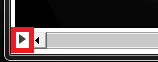
\includegraphics[width=0.3\textwidth]{mod1-publishing/figures/stack-animation-button.png}%
		}
		\medskip
		\captionof{figure}{Start stack animation.}\label{fig:stack-animation-button}
		\end{center}
	\end{minipage}
	
	\item Using the stack toolbar (Fig. \ref{fig:stack-toolbar}), you can \texttt{[Start Animation]} and \texttt{[Stop Animation]} as well.
	
	\begin{minipage}[t]{\linewidth}
		\begin{center}
		\adjustbox{valign=t}{%
			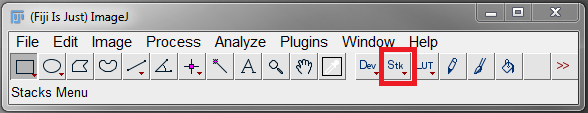
\includegraphics[width=0.7\textwidth]{mod1-publishing/figures/stack-toolbar.png}%
		}
		\medskip
		\captionof{figure}{Stacks toolbar.}\label{fig:stack-toolbar}
		\end{center}
	\end{minipage}
	
	\item Use the \texttt{[Animation Options]} from the stack toolbar to increase the animation speed to 20 fps (frames-per-second) and loop back and forth. The animation should look much smoother now (Fig. \ref{fig:animation-options-dialog}).
	
	\begin{minipage}[t]{\linewidth}
		\begin{center}
		\adjustbox{valign=t}{%
			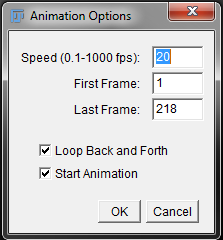
\includegraphics[width=0.4\textwidth]{mod1-publishing/figures/animation-options-dialog.png}%
		}
		\medskip
		\captionof{figure}{Stacks toolbar.}\label{fig:animation-options-dialog}
		\end{center}
	\end{minipage}
	
	SAVE AS AVI!!
	
\end{enumerate}

\end{taskbox}

It is possible that the image data you import has the dimensions mixed up. If the data is a stack, you can use \texttt{[Image > Properties]} to reorder channels, slices and frames. However, it is more flexible to convert the stack to a hyperstack and perform re-ordering on the hyperstack.

\begin{taskbox}{Order of Dimensions}

\begin{enumerate}
	\item Open the file flybrain-template.tif in /mod1-publishing/data if it is not still open.
	\item Use \texttt{[Image > Hyperstacks > Stack to Hyperstack...]} to convert the stack to a hyperstack. In our test image, the order, channels, slices and frames should be detected correctly. 
	\item Now, you can easily re-order the dimensions of the hyperstack using \texttt{[Image > Hyperstacks > Re-order Hyperstacks...]}. Although this does not make any sense, change the z-dimension to a time dimension. As you can see, from the user perspective, this does not change anything at the moment.
\end{enumerate}

\end{taskbox}

Fiji offers many ways to manipulate (hyper)stacks. You can concatenate, combine, interleave, insert or split stacks; convert images to stacks and back, remove and add slices, make substacks, create a montage or generate a stack from a montage. These functions can be found under \texttt{[Image > Stacks]} and especially \texttt{[Image > Stacks > Tools]}. 

\begin{taskbox}{Manipulating Stacks -- Creating a Montage}
A common way 3-dimensional data is presented (typically along time or z-axis) is the montage view.

\begin{enumerate}
	\item Open the file flybrain-template.tif in /mod1-publishing/data if it is not still open.
	\item Use \texttt{[Image > Stacks > Make Montage...]}. In the dialog, set \texttt{[Columns]} and \texttt{[Rows]} to 5, \texttt{[First Slice]} to 100, \texttt{[Last Slice]} to 124, change the \texttt{[Border Width]} to 1 pixel and tick \texttt{[Label Slices]} (Fig. \ref{fig:make-montage-dialog}).
	
	\begin{minipage}[t]{\linewidth}
		\begin{center}
		\adjustbox{valign=t}{%
			\includegraphics[width=0.4\textwidth]{mod1-publishing/figures/make_montage_dialog.png}%
		}
		\medskip
		\captionof{figure}{Make Montage Dialog.}\label{fig:make-montage-dialog}
		\end{center}
	\end{minipage}
	
	\item You can see how easy it is to create a custom montage view, play with the different options, e.g. \texttt{[Increment]}.
\end{enumerate}

\end{taskbox}

\begin{taskbox}{Manipulating Stacks -- Creating an Insert}
We now want to do something more complicated: let's say we want to show a detail of the flybrain, e.g. the central complex or the optic lobes. To help viewers, we want to put a little version of the complete brain in the corner of our 3D image as an overview. How would you proceed?

\begin{enumerate}
	\item Open the file flybrain-template.tif in /mod1-publishing/data if it is not still open.
	\item Use the rectangle tool to select an interesting part of the brain that you want to highlight. Duplicate the complete stack using \texttt{[Image > Duplicate]}, this will only duplicate the part you selected. 
	\item Use \texttt{[Image > Adjust > Size...]} to create an image with 1024 pixel width and no interpolation.
	\item Go back to our original image of the fly brain and use \texttt{[Image > Scale...]} to reduce the image size to 20\% (x, y) with bilinear interpolation.
	\item The insert is created with \texttt{[Image > Stacks > Tools > Insert...]}. Make sure you use the detailed view of brain as \texttt{[Destination]} and the overview as \texttt{[Source]}. \texttt{[X-Location]} and \texttt{[Y-Location]} can remain 0 (Fig. \ref{fig:stack-inserter-dialog}).
	
	\begin{minipage}[t]{\linewidth}
		\begin{center}
		\adjustbox{valign=t}{%
			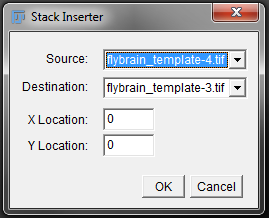
\includegraphics[width=0.4\textwidth]{mod1-publishing/figures/stack-inserter-dialog.png}%
		}
		\medskip
		\captionof{figure}{Stack Inserter Dialog.}\label{fig:stack-inserter-dialog}
		\end{center}
	\end{minipage}
	
	\item Again, a very easy procedure -- explore further stack operations on your own.
\end{enumerate}

\end{taskbox}

\subsection{Color images}

So far, we only analyzed images with one color channel (grayscale), i.e. at each spatial position, we only had one pixel with one value. In microscopy, we often encounter multi-channel images where each channel corresponds to one modality. One channel for each fluorophore intensity, a channel for a DIC image or even a channel that does not represent brightness but for example fluorophore lifetime. Outside microscopy, we also usually encounter color images, these are often RGB images that consist of red, green and blue 8-bit channels. Again, publisher demands on the color usage varies, sometimes they demand that the RGB color space you usually work with on your computer is converted to the CMYK color space that is typically used in print. Luckily, as the primary source for distributing and viewing a publication are various digital devices, conversion demands become less common.

\minisec{Color models}
Outside microscopy, two colorspaces are very common:
\begin{enumerate}
	\item RGB (Red Green Blue)\\A single RGB image has three, fixed color channels: red, green and blue. Each of those have a fixed bit-depth of 8-bit, resulting in a single RGB image with 24-bit. These colors have been chosen as computer screens generate colors by mixing red, green and blue light and therefore, RGB images directly determine how much of each color to use but are device dependent (actually, RGB is based on human color perception).
	\item CMYK (Cyan Magenta Yellow Key)\\A single CMYK image is based on four colors: cyan, magenta, yellow and black. The color model is primarily used in printing, but is device-dependent as well. When you want to publish a manuscript, it is very likely that you will be asked to convert your figures to the CMYK color space. This can be done with Fiji using existing Plugins, but it might be better to perform the conversion for the total final figure when all other editing has been finished. As the online versions of publications have become much more important than the actual prints, efforts to produce color-true conversions for printing become much less important.
\end{enumerate}

\begin{taskbox}{RGB Images}

\begin{enumerate}
	\item Open the file muscle-cell.tif in /mod1-publishing/data\footnote{This image was taken from a publication in Nature Cell Biology 5, 598(2003); Cell of the Month: The vascular smooth muscle cell cytoskeleton; Mario Gimona; DOI:10.1038.ncb0703-598}. This is a RGB image of a mouse smooth muscle cell with fluorescent labels of the cytoskeleton. Use \texttt{[Image > Show Info...]} for details about this image.
	\item Use \texttt{[Image > Adjust > Brightness/Contrast]} and change the slider values. Observe that this operation affects all colors simultaneously. Reset the changes.
	\item We now split the red, green and blue channels of the RGB image with \texttt{[Image > Color > Split Channels]}. Three windows appear, each showing the respective color content. 
	\item Let's combine these channels again with \texttt{[Image > Color > Merge Channels]}. The merge-function gives us many options to create a merged image (Fig. \ref{fig:merge_channels_dialog}). Do not set any options and use the same color channels.
	
	\begin{minipage}[t]{\linewidth}
		\begin{center}
		\adjustbox{valign=t}{%
			\includegraphics[width=0.4\textwidth]{/mod1-publishing/figures/merge_channels_dialog.png}%
		}
		\medskip
		\captionof{figure}{Merge Channels Dialog.}\label{fig:merge-channels-dialog}
		\end{center}
	\end{minipage}
	
	\item Now split again and merge back, but with option \texttt{[Create composite]} ticked. This creates a slider below the image, indicating that we created a three-layered stack, one layer for each color.  
	\item The composite image allows us to work on each channel separately. Perform \texttt{[Image > Color > Channels Tool...]}. In this dialog, you can select individual channels in composite mode or view individual channels in Color/Grayscale mode (Fig. \ref{fig:channels-tool-dialog}). Try out the different settings.
	
		\begin{minipage}[t]{\linewidth}
		\begin{center}
		\adjustbox{valign=t}{%
			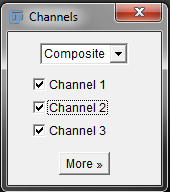
\includegraphics[width=0.4\textwidth]{figures/chapter1/channels-tool-dialog.png}%
		}
		\medskip
		\captionof{figure}{Channels Tool Dialog.}\label{fig:channels-tool-dialog}
		\end{center}
	\end{minipage}
	
	\item Try to perform already know operations on just one color channel, e.g. Adjust the brightness (you can see that the little histogram changes color when you change the channel!).
\end{enumerate}

\end{taskbox}

\begin{taskbox}{Convert RGB to CMYK -- Extending Fiji with Plugins}
Although Fiji has a great core functionality included, the power of this tool can only be appreciated with the many existing macros and plugins. While some plugins are already included in the Fiji distribution, you most likely will encounter some function you need that is not included -- and if this is a common task it is very likely that someone already solved this problem. 

\begin{enumerate}
	\item Convert the composite image back to a RGB image with \texttt{[Image > Color > Stack to RGB]}.
	\item We now want to convert the RGB image into a CMYK image for publication. However, Fiji is not able to do so and we have to extend the functionality. A quick search ('imagej convert to cmyk') shows that, fortunately, Stephan Saalfeld and Wayne Rasband wrote a plugin for this (two names you might encounter more often).
	\item You can find the file RGB\_to\_CMYK.class in the folder mod1-publishing/data/. Installing this plugin is very easy, just drag and drop the file onto the main Fiji window. You are asked to save the file in the plugins directory of Fiji. 
	\item Convert the image to CMYK with \texttt{[Plugins > RGB to CMYK]}.
\end{enumerate}

\end{taskbox}

\minisec{Lookup Tables}
For a computer, an image is a matrix with the same dimensions as the image and the range of possible values at each matrix position are determined by the bit-depth. A \emph{lookup table (LUT)} maps these values to a color/brightness that is displayed on the screen. Often, the LUT is simply called \emph{colormap}. The default LUT is gray-scale that, in an 8-bit image, assigns black to zero and white to 255. Intermediate values are represented as gray-levels and the same idea applies to any bit-depth.
The advantage using a LUT is obvious; we can create arbitrary LUTs with any coloring we want. These colored LUTs are called 'pseudo-color'. These LUTs are typically used to indicate fluorophore emission wavelengths but are sometimes changed to emphasize certain aspects of the data.

Figure \ref{fig:lookup_tables} shows the LUTs available in Fiji, the figure was created by the command \texttt{[Image > Color > Display LUTs]}. Very common LUTs are \emph{grayscale}, \emph{spectrum}, \emph{fire} and \emph{physics}.

% Module 2: Measuring intensities
\chapter{Measuring intensities}
An image contains one type of information: the intensities of the pixels in the image. In this chapter, we will show you how to work with this intensity information in a quantitative way. We will look at intensity distributions and how to perform measurements based on the intensity distributions in regions of the image (e.g. a cell). 

\section{Histograms}
Each pixel in an image has an intensity (a pixel value). The intensity histogram of an image is a plot that shows the distribution of pixel counts over a range of intensity values, typically the bit-depth of the image or the range between the minimum and maximum values within the image. The histogram can be used to examine the signal and background levels (useful when you want to identify objects of interest).

\begin{taskbox}{Working with histograms}
\begin{enumerate}
	\item Open the image hela-cells.tif in /mod2/data. This is another standard Fiji sample image showing HeLa cells. Lysosomes are red, mitochondria green and the nucleus blue. 
	\item We can show the histogram with \texttt{[Analyze > Histogram]}. The histogram is displayed in a new window (Fig. \ref{fig:histogram}). The x-axis shows the pixel value and the y-axis the count. Note that the histogram refers to the channel that was active when the command was called.
	
	\begin{minipage}[t]{\linewidth}
		\begin{center}
		\adjustbox{valign=t}{%
			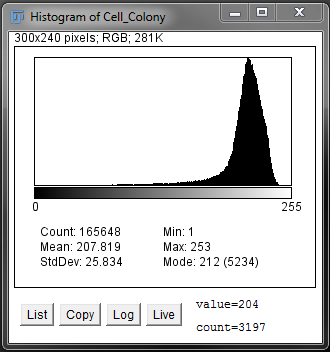
\includegraphics[width=0.4\textwidth]{mod2/figures/histogram.png}%
		}
		\medskip
		\captionof{figure}{Histogram.}\label{fig:histogram}
		\end{center}
	\end{minipage}
	
	\item Obtain the highest and lowest intensities from the histogram. What does the histogram range tell you?
	\item Click on [list] to obtain a list with values and counts. [Log] displays the same histogram on a log-scale.
	\item Click on [live] in the histogram dialog and change the channel. Observe the changes in the histogram and note the color changes in the depicted colormap bar.
	
\end{enumerate}

\end{taskbox}

\section{ROIs and the ROI Manager}
We now introduce a very powerful concept that is widely used for many types of analyses - the region of interest. Many operations can be applied to parts of the image when a region is selected by \emph{ROI} (region-of-interest) tools. The shape of the ROI is arbitrary; it can consist of a geometric shape, such as a circle or a line, but can be any selection of pixels. You already used ROIs when you selected a line or a point! Next, we will cover some basic ROI operations.

\begin{taskbox}{Working with ROIs}

One of the operations you can perform on a ROI is cropping:
\begin{enumerate}
	\item Open any image. Duplicate the image. Select a region by a rectangular ROI. Then, perform \texttt{[Image > Crop]} on the duplicate. Close the cropped image.
	\item Duplicate the original image again. Use the freehand selection to create a ROI on the duplicate. Crop the image. Note that the minimum and maximum values of your ROI have been used to determine a rectangular selection for the cropping.
\end{enumerate}

ROIs can be used to create image masks. An image masks is a binary image that define which parts of the image to analyze or measure.

\begin{enumerate}
	\item Open any image. Duplicate the image. Create a few circular ROIs (press <shift> during creation to keep multiple ROIs). 
	\item Use \texttt{[Edit > Clear Outside]} and then \texttt{[Edit > Fill]} to generate a mask image (this should look similar to fig. \ref{fig:binary-mask}. The 'Clear' command fills the respective area with the background color, 'fill' with the foreground color.
	
	\begin{minipage}[t]{\linewidth}
		\begin{center}
		\adjustbox{valign=t}{%
			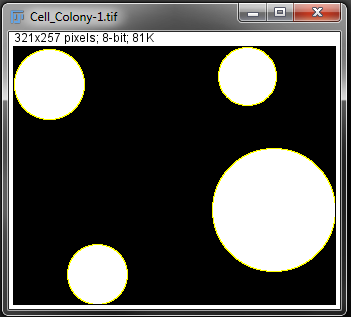
\includegraphics[width=0.4\textwidth]{mod2/figures/binary-mask.png}%
		}
		\medskip
		\captionof{figure}{Example binary mask.}\label{fig:binary-mask}
		\end{center}
	\end{minipage}
	
	\item Undo what you have done with \texttt{[Edit > Undo]}. You will notice that, in contrast to other programs, Fiji only allows to undo the most recent operation. This is done to minimize memory consumption. \texttt{[File > Revert]} allows you to go back to the last saved state.
	\item Go back to the original image. Use the command \texttt{[Edit > Selection > Create Mask]} to directly generate a mask image.
\end{enumerate}

Operations are usually performed on the selected ROIs and on the whole image if no selections exist. 
\begin{enumerate}
	\item Open any image. Duplicate the image. Select any ROI you like. 
	\item Observe that \texttt{[Edit > Invert]} only affects the selected pixels. Undo the inversion.
\end{enumerate}

Finally, there are several operations that work on a ROI itself without changing pixel values \texttt{[Edit > Selection > ...]}, see fig. \ref{fig:selection-options}. Let us explore a few of those options.

\begin{minipage}[t]{\linewidth}
		\begin{center}
		\adjustbox{valign=t}{%
			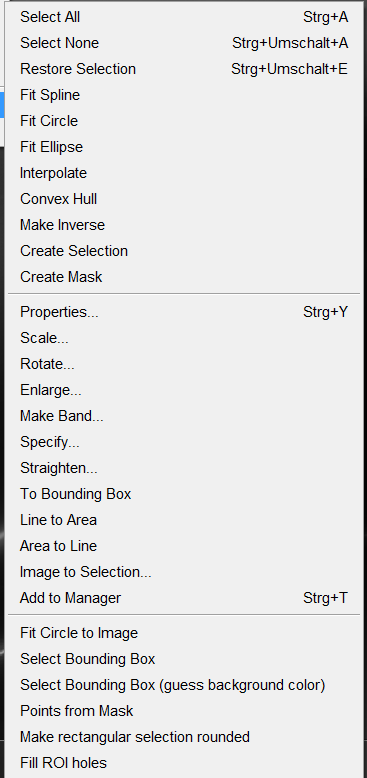
\includegraphics[width=0.4\textwidth]{mod2/figures/selection-options.png}%
		}
		\medskip
		\captionof{figure}{Selection options.}\label{fig:selection-options}
		\end{center}
	\end{minipage}


\begin{enumerate}
	\item Open an image, duplicate and draw a freehand selection with an outline that includes inner parts that are not selected. Fit a spline \texttt{[Fit Spline]}. This creates a smoothed version of the selection where individual points can now be dragged around and the shape can be changed. This can be useful to correct the outline of a shape (e.g. a worm or a cell). 
	\item Use \texttt{[To Bounding Box]}. This creates a rectangular region that just fits over the selection (this is the same as the crop area). Undo the last operation.
	\item Use \texttt{[Convex Hull]}. This creates an outline of the selection, where a straight line between every pair of points within the ROI is also within the ROI (Definition of a convex object in Euclidean space). This can be useful if you want to measure the extent of an object with an irregular shape. Undo the last operation.
	\item Explore the operations \texttt{[Scale]}, \texttt{[Make Inverse]}, \texttt{[Enlarge]} and \texttt{[Rotate]}.
	\item Each ROI has properties that can be displayed and changed with \texttt{[Properties]}. Especially useful when you work with multiple ROIs (and the ROI Manager, see below), can be ROI names (Fig. \ref{fig:roi-properties}). If you need the ROI coordinates outside Fiji, you can list the coordinates of the ROI as well.
	
	\begin{minipage}[t]{\linewidth}
		\begin{center}
		\adjustbox{valign=t}{%
			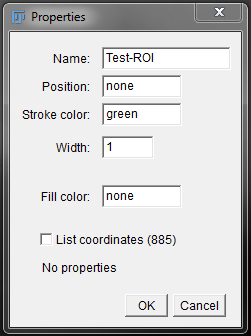
\includegraphics[width=0.4\textwidth]{mod2/figures/roi-properties.png}%
		}
		\medskip
		\captionof{figure}{ROI properties.}\label{fig:roi-properties}
		\end{center}
	\end{minipage}
	
\end{enumerate}

\end{taskbox}

\minisec{Managing multiple ROIs}
Fiji has an ROI manager to assist when you work with multiple ROIs. Open the ROI manager with \texttt{[Analyze > Tools > ROI Manager...]}. The manager allows you to add, delete and modify existing ROIs, save and load ROI coordinates, and change their display properties (Fig. \ref{fig:roi-manager}).

\begin{figure}[!ht]
	\begin{center}
		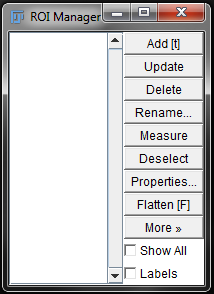
\includegraphics[width=0.3\textwidth]{mod2/figures/roi-manager.png}
		\caption{ROI manager.}\label{fig:roi-manager}
	\end{center}
\end{figure}

\begin{taskbox}{Working with the ROI Manager}
\begin{enumerate}
	\item Open the image hela-cells.tif in /mod2/data.
	\item Open the ROI Manager with \texttt{[Analyze > Tools > ROI Manager...]}.
	\item For the following analysis, we will only work on the bottom-most cell. Select the blue channel showing the nucleus. Use the ROI tools to create an accurate outline of the nucleus and add the selected region to the ROI manager. Rename the ROI to 'Nucleus'.
	\item Select the blue channel showing the mitochondria. In this channel, we can estimate the cell outline - create the outline and add the selected region to the ROI manager, rename ROI to 'Cell'.
	\item Let's say the task we want to solve is get the area of the cell, excluding the nucleus, for our further analysis. We now explore an option using the ROI manager, we will later explore another way using masks and image math. Select 'Nucleus' and 'Cell ROIs simultaneously. Then go to the [More>>] button and select the XOR operation. 
\emph{XOR} is the \emph{exclusive or} (exclusive disjunction). This is a logical operation that we apply to the ROIs. The XOR function returns the area where both inputs differ, i.e. not overlap. As the 'nucleus' ROI is located within the 'Cell' ROI, this subtracts the nucleus from the cell. Add the resulting ROI to the ROI Manager and rename to 'Cytoplasm'.
	\item Select all ROIs and save them on disk - we will use these ROIs for measurements. 
\end{enumerate}

\end{taskbox}

\section{Measurements}

The easiest way to read pixel values is moving the mouse pointer over individual pixels and reading their intensity value in the main Fiji bar. The histogram allows us to get the distribution of pixel intensities. Fiji has the function \texttt{[Analyze > Measure]} to obtain statistical information about pixel values within a ROI. \texttt{[Analyze > Set Measurements...] }allows us to select the parameters we want to measure. For example, following parameters can be obtained (Fig. \ref{fig:set_measurements-dialog}):
\begin{description}
	\item[Area] Area of selection in square pixels. If the image is calibrated, Area is displayed in according units.
	\item[Standard Deviation] Standard deviation of intensity values.
	\item[Min and Max Gray Value] Minimum and maximum intensities in selection.
	\item[Center of mass] Intensity-weighted spatial average.
	\item[Bounding rectangle] Bounding box, smallest rectangle enclosing selection.
	\item[Area fraction] The percentage of highlighted pixels, or the percentage of non-zero pixels.
	\item[Mean gray value] Mean intensity in selection.
	\item[Centroid] The average of all \emph{x} and \emph{y} coordinates in the selection.
	\item[Perimeter] The length of the outside boundary of the selection.
\end{description}

\begin{figure}[!ht]
	\begin{center}
		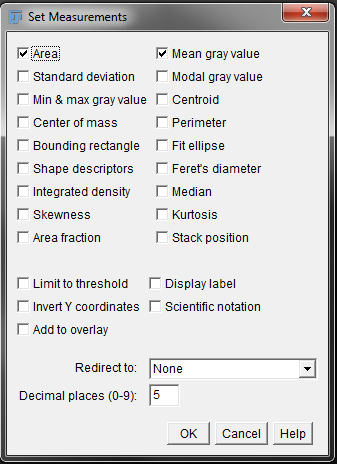
\includegraphics[width=0.4\textwidth]{mod2/figures/set-measurements-dialog.png}
		\caption{Set Measurements Dialog.}\label{fig:set-measurements-dialog}
	\end{center}
\end{figure}

\begin{taskbox}{Using the ROI Manager}
Now, we are going to combine ROIs (and the ROI Manager) with measurements -- you will see how powerful this already gets!
\begin{enumerate}
	\item Open the image hela-cells.tif in /mod2/data. Open the ROI Manager and load the previously generated ROI data.
	\item Measure the area and average intensity of the whole cell, the nucleus and the cytoplasm in the green channel and compare the results (Fig. \ref{fig:results-window}).
	
		\begin{minipage}[t]{\linewidth}
		\begin{center}
		\adjustbox{valign=t}{%
			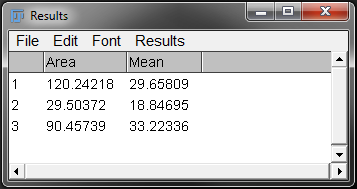
\includegraphics[width=0.3\textwidth]{mod2/figures/results-window.png}%
		}
		\medskip
		\captionof{figure}{Results window showing measurements.}\label{fig:results-window}
		\end{center}
	\end{minipage}
	
	\item Create a ROI in the background of the image (no cell), select the green channel and measure the average intensity again. Name the ROI 'Background' and update the saved ROI file; we will need this for further measurements.
\end{enumerate}	
\end{taskbox}

\section{Changing pixel intensities}
We now have seen various times that an image is represented as a matrix and that we can operate on individual pixels. In this section, we explore basic operations that allow us to modify the values of individual pixels in a ROI or the whole image. As you will see, you have to be careful with these operations, especially when you want to measure and/or compare intensities. However, they can be extremely useful to identify interesting regions of your images or enhance details.

\subsection{Arithmetic}
As an image is a matrix of numbers, we can do usual math on those pixels. We will go through one example where this might be useful and one example to show that things can go wrong if we are not careful.

\begin{taskbox}{Subtracting background levels}
A common task is the subtraction of the background levels of our images to make them comparable (background levels might vary). Subtracting a constant is the most basic background subtraction possible. 

\begin{enumerate}
	\item Open the image hela-cells.tif in /mod2/data. Open the ROI Manager and load the previously generated ROI data that includes the background ROI.
	\item Measure the average intensity in the background and note the value.
	\item Select the overall image \texttt{[Edit > Selection > Select All]} in the green channel. 
	\item Subtract the average background level from the green channel, using \texttt{[Process > Math > Subtract]}. You can also measure the backgrounds of the other color channels and subtract those as well.
\end{enumerate}

\end{taskbox}

\begin{taskbox}{Bit-depth/Format Problems}
A common task is the subtraction of the background levels of our images to make them comparable (background levels might vary). Subtracting a constant is the most basic background subtraction possible. 

\begin{enumerate}
	\item Open the image hela-cells.tif in /mod2/data. Duplicate the green channel.
	\item Look at the histogram of the green channel.
	\item Now, multiply the image by 2.5 - this increases the brightness of the image. 
	\item Generate the histogram again and compare the number of saturated values. As you can see, if the resulting value of a pixel is clipped if we get a value outside our bit-depth. If the result is a real number but our format only allows whole numbers, the resulting value would be rounded. Of course, this was a rather stupid example, but this is a common mistake when you perform more complicated calculations on your images.
	\item if you want, you can convert your image to an appropriate format and compare results.
	\item You can also try to perform the previous invert-example without the conversion to 32-bit.
	\end{enumerate}
	
\end{taskbox}

\subsection{Doing math with two images}
In the previous section, we operated with a single image and constant numeric values. Likewise, we can perform computations that involve two images. Assuming that both images have the same dimensions, we can perform calculations on each pair of pixels at the same position. For example, this type of operation can be used to subtract an image showing only (non-uniform) background from the image showing background + data or we can compare two images by obtaining their difference.

\begin{taskbox}{Background subtraction}
In this example, we are exploring a common method to subtract background information from a time-series. In the given example, we have moving bacteria that were imaged with phase contrast microscopy. The key idea for the background subtraction is that on each pixel, most of the time no bacteria is visible. We therefore create an average image and subtract this image from the original images to increase contrast of moving bacteria.

\begin{enumerate}
	\item Open the image bacteria-tracks.tif in /mod2/data. This image was create from supplementary video 1 of the publication: Rosser et al. (2013) Novel Methods for Analysing Bacterial Tracks Reveal Persistence in Rhodobacter sphaeroides, PLOS Computational Biology, DOI: 10.1371/journal.pcbi.1003276. Please note that this was not the original data, it seems that the supplementary movie was compressed!
	\item Perform a Z-projection to create an average image.
	\item Use \texttt{[Process > Image Calculator...]} to subtract the average image from each image in the original time-series and display the difference in a new window.
	\item Do you see any differences?
\end{enumerate}

Not surprisingly, the authors of the original publication used exactly this approach as the first step in their image processing.

\end{taskbox}

\begin{taskbox}{Math on Masks}
Before, we used the ROI Manager XOR function to obtain the cytoplasm ROI. We can obtain the same result using image masks and image calculations (actually this is likely happening behind the scenes anyway!).

\begin{enumerate}
	\item Open the image hela-cells.tif in /mod2/data. Open the ROI Manager and load the previously generated ROI data that includes the background ROI.
	\item Duplicate just the green channel.
	\item Select the Nucleus ROI and create a mask (look at the previous exercise if you forgot how to proceed). Duplicate the mask.
	\item Now, select the Cell ROI and create another mask.
	\item you should now have two image masks (black-and-white images, see fig. \ref{fig:image-masks}).	
	
		\begin{minipage}[t]{\linewidth}
		\begin{center}
		\adjustbox{valign=t}{%
			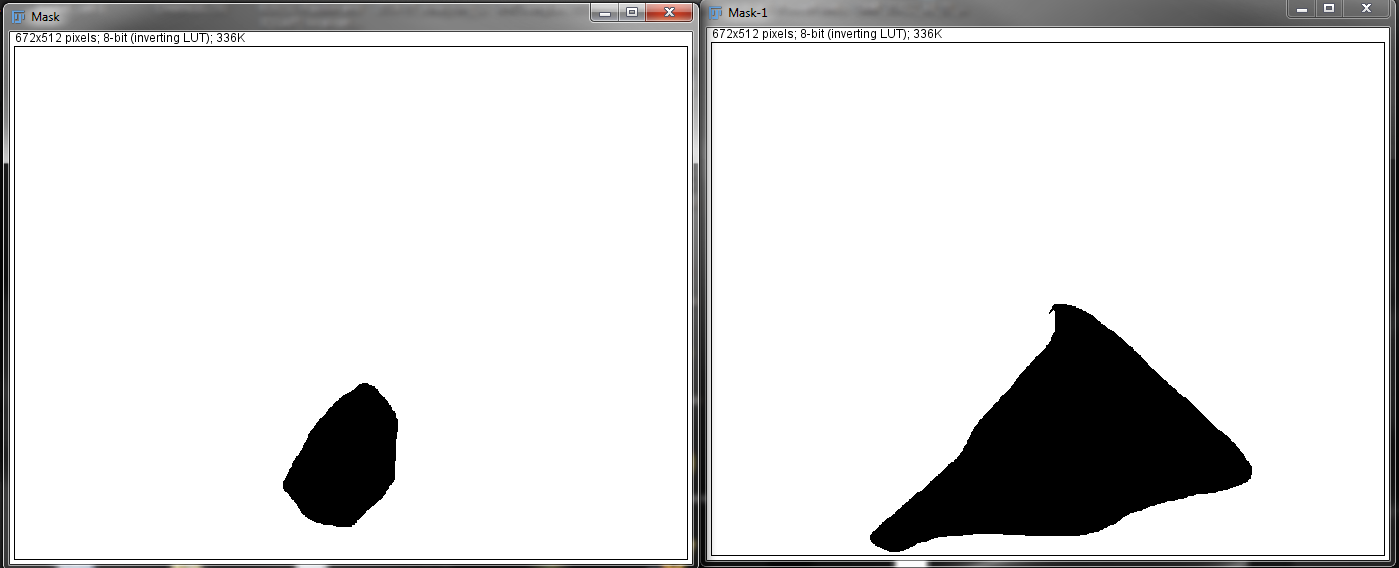
\includegraphics[width=0.8\textwidth]{mod2/figures/image-masks.png}%
		}
		\medskip
		\captionof{figure}{Image Masks.}\label{fig:image-masks}
		\end{center}
	\end{minipage}
	
	\item Calculate the XOR function using the binary data of both images (\texttt{[Process > Image Calculator...]}).
	\item Compare the results with the cytoplasm ROI.
	\item Using \texttt{[Edit > Create Selection]}, you can create a selection from the mask.
\end{enumerate}

\end{taskbox}

\section{Contrast enhancements}
You might already have experience with contrast enhancing of digital images, since most photo-editing software/apps have this function. Low contrast images have small differences in tones and objects are difficult to observe. If the contrast is too high, the tone difference is very high, the picture is 'over-exposed'. Contrast can be adjusted to optimize the appearance of the image. Contrast enhancement primarily changes the LUT, leaving the original data unaffected (it is affected if you apply the changes). Contrast enhancement should be used with care as pixel values are altered and intensity calculations become useless. Therefore, you should avoid contrast enhancements when you analyze intensities (this also applies to the figures that make your point!). Even if you treat all images the same way, you have to make sure that you avoid clipping and that results are not distorted by contrast enhancement.

\begin{taskbox}{Contrast Enhancement and Image Manipulation}
Let's assume you want to show gel data in your manuscript. After performing following steps, can you discuss why contrast enhancement might be considered fraud?
\begin{enumerate}
	\item Open the image gel.tif in mod2/data and duplicate the image (another Fiji sample image).
	\item Adjust Contrast and Brightness and compare images. What is the problem with the contrast-enhanced image (Fig. \ref{fig:contrast-problem})?
	
	\begin{minipage}[t]{\linewidth}
		\begin{center}
		\adjustbox{valign=t}{%
			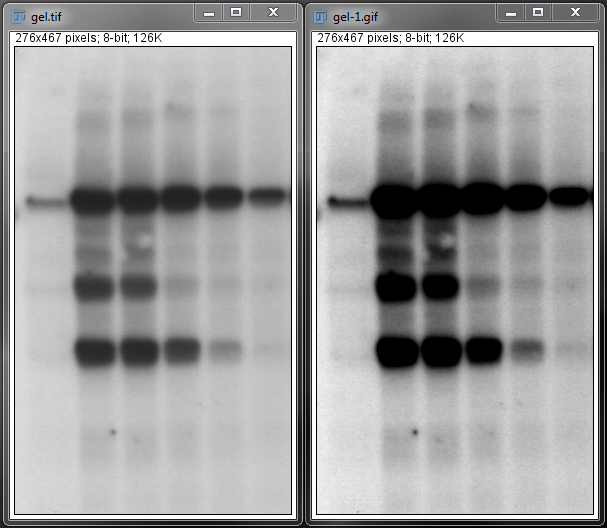
\includegraphics[width=0.8\textwidth]{mod2/figures/contrast-problem.png}%
		}
		\medskip
		\captionof{figure}{Contrast enhancement. The left gel plot shows the original data. Contrast enhancement in the right gel plot shows that you interpretation of this gel might be different.}\label{fig:contrast-problem}
		\end{center}
	\end{minipage}
	
	\end{enumerate}
\end{taskbox}

\subsection{Histogram Normalization}
With normalization, pixel values are normalized according to the minimum and the maximum pixel values in the image and bit-depth. If the minimum pixel value is \emph{pmin} and the maximum is \emph{pmax} in an 8-bit image, then normalization is done as follows:

\begin{equation*}
\mathit{NewPixelValue}=\frac{(\mathit{OriginalPixelValue}-\mathit{pmin})}{(\mathit{pmax}-\mathit{pmin})}\ast
255
\end{equation*}

\begin{taskbox}{Histogram Normalization}

\begin{enumerate}
	\item Open the image hela-cells.tif in /mod2/data and duplicate the green channel. Obtain a histogram.
	\item Use \texttt{[Process > Enhance Contrast]} on the duplicate. Set saturated pixels to 0, tick normalize and not equalize (Fig. \ref{fig:enhance-contrast-dialog}) and obtain a histogram afterwards.
	
	\begin{minipage}[t]{\linewidth}
		\begin{center}
		\adjustbox{valign=t}{%
			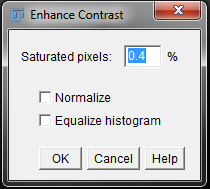
\includegraphics[width=0.3\textwidth]{mod2/figures/enhance-contrast-dialog.png}%
		}
		\medskip
		\captionof{figure}{Enhance Contrast Dialog.}\label{fig:enhance-contrast-dialog}
		\end{center}
	\end{minipage}
	
	\item Compare the histograms. 
	\item Leave the images open; you can also explore different settings.
	
	\end{enumerate}
\end{taskbox}

\subsection{Histogram Equalization}
Equalization converts pixel values so that the values are distributed evenly within the dynamic range. 

\begin{taskbox}{Histogram Equalization}

\begin{enumerate}
	\item Go to the original image showing the green channel.
	\item Use \texttt{[Process > Enhance Contrast]} on the duplicate. Set saturated pixels to 0, tick equalize, not normalize and obtain a histogram.
	\item Compare the histograms. 
	
	\end{enumerate}
\end{taskbox}

\subsection{Local Histogram Equalization}
Histogram equalization could also be performed on a local basis. This becomes powerful, as more local details could be contrast enhanced. In Fiji, you can use local histogram equalization with \texttt{[Process > Enhance Local Contrast (CLAHE)]}.

\section{Colocalization}



\bibliographystyle{plainnat}
%\bibliography{coursebib}


\end{document}





